% Figure 5.6. Load parameters checked against cases.toml, 2026-09-07.
% 2026-09-28: traction drawn flush with the right edge (no outward offset), Gamma_t label
% moved inside the domain, redundant top "free" annotation removed.
\documentclass[tikz,border=5pt]{standalone}
\usepackage{amsmath}
\usetikzlibrary{arrows.meta}
\definecolor{loadred}{RGB}{185,35,35}
\begin{document}
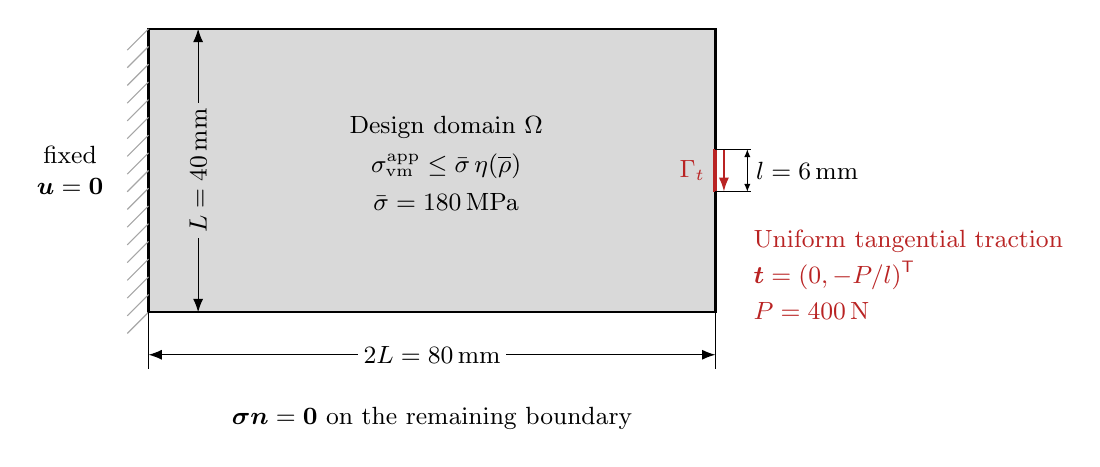
\begin{tikzpicture}[x=0.09cm,y=0.09cm,>=Latex,font=\small,
load/.style={loadred,thick,-{Latex[length=1.8mm,width=1.3mm]}}]
\draw[thick,fill=black!15] (0,0) rectangle (80,40);
\foreach \y in {0,2.5,...,40} \draw[gray!70] (0,\y) -- (-3,\y-3);
\node[anchor=east,align=center] at (-5,20) {fixed\\$\boldsymbol u=\boldsymbol 0$};
\node[align=center] at (42,21) {Design domain $\Omega$\\[3pt]
$\sigma_{\mathrm{vm}}^{\mathrm{app}}\leq\bar\sigma\,\eta(\overline\rho)$\\[3pt]
$\bar\sigma=180\,\mathrm{MPa}$};
\draw[thin,<->] (7,0) -- (7,40)
node[midway,fill=black!15,rotate=90,inner sep=2pt] {$L=40\,\mathrm{mm}$};
\draw[thin] (0,0) -- (0,-8);
\draw[thin] (80,0) -- (80,-8);
\draw[thin,<->] (0,-6) -- (80,-6)
node[midway,fill=white,inner sep=2pt] {$2L=80\,\mathrm{mm}$};
% Loaded segment Gamma_t: x=80, y in [17,23]. Tangential traction points downward and is
% drawn flush with the edge; the arrow spans exactly the loaded length.
\draw[loadred,line width=1.4pt] (80,17) -- (80,23);
\draw[load] (81.2,23) -- (81.2,17);
\node[loadred,anchor=east,inner sep=1pt] at (79,20) {$\Gamma_t$};
% Dimension lines refer to the loaded segment endpoints.
\draw[thin] (80,17) -- (85,17);
\draw[thin] (80,23) -- (85,23);
\draw[thin,<->,>= {Latex[length=1mm,width=0.8mm]}] (84.5,17) -- (84.5,23)
node[midway,right,inner sep=3pt] {$l=6\,\mathrm{mm}$};
\node[loadred,align=left,anchor=north west] at (84,13)
{Uniform tangential traction\\[2pt]
$\boldsymbol t=(0,-P/l)^{\mathsf T}$\\[2pt]
$P=400\,\mathrm{N}$};
\node[align=center,anchor=north] at (40,-12)
{$\boldsymbol\sigma\boldsymbol n=\boldsymbol 0$ on the remaining boundary};
\end{tikzpicture}
\end{document}
